We need a more systematic and rigorous way to describe the interaction of threads through memory, their use of the shared data, and its effect on concurrent applications. This description is known as the memory model. The memory model describes what guarantees and restrictions exist when threads access the same memory location.

Prior to the C++11 standard, the C++ language had no memory model at all (the word thread was not mentioned in the standard). Why is that a problem? Consider our producer-consumer example again (let us focus on the producer side):

\begin{lstlisting}[style=styleCXX]
std::mutex mN;
size_t N = 0;
…
new (buffer + N) T( … arguments … );
{ // Critical section start – acquire lock
	std::lock_guard l(mN);
	++N;
} // Critical section end - release lock
\end{lstlisting}

The lock\_guard is just an RAII wrapper around the mutex, so we can't forget to unlock it, so the code boils down to this:

\begin{lstlisting}[style=styleCXX]
std::mutex mN;
size_t N = 0;
…
new (buffer + N) T( … arguments … ); // N
mN.lock(); // mN
++N; // N
mN.unlock(); // mN
\end{lstlisting}

Note that each line of this code uses either the variable N or the object nM, but they are never used together in one operation. From the C++ point of view, this code is similar to the following:

\begin{lstlisting}[style=styleCXX]
size_t n, m;
++m;
++n;
\end{lstlisting}

In this code, the order of the operations does not matter, and the compiler is free to reorder them as long as the observable behavior does not change (observable behavior is things like input and output, changing a value in memory is not an observable behavior). Going back to our original example, why doesn't the compiler reorder the operations there?

\begin{lstlisting}[style=styleCXX]
mN.lock(); // mN
mN.unlock(); // mN
++N; // N
\end{lstlisting}

This would be very bad, and yet, nothing in the C++ standard (until C++11) prevents the compiler from doing so.

Of course, we were writing multi-threaded programs in C++ long before 2011, so how did they work? Obviously, the compilers did not do such optimizations, but why? The answer is found in the memory model: the compilers provided certain guarantees that went beyond the C++ standard and supplied a certain memory model even when the standard required none. The Windows-based compilers followed the Windows memory model, while most Unix- and Linux-based compilers provided the POSIX memory model and the corresponding guarantees.

The C++11 standard changed that and gave C++ its own memory model. We have already taken advantage of it in the previous section: the memory order guarantees that accompany the atomic operations, and the locks are part of this memory model. The C++ memory model now guarantees portability across platforms that previously offered a different set of guarantees, each according to its memory model. In addition, the C++ memory model offers some language-specific guarantees.

We have seen these guarantees in the form of the different memory order specifications: relaxed, acquire, release, and acquire-release. C++ has an even stricter memory order called sequentially consistent (std::memory\_order\_seq\_cst), which is the default order you get when you don't specify one: not only there is a bidirectional memory barrier associated with each atomic operation that specifies this order, but the entire program satisfies the sequential consistency requirement. This requirement states that the program behaves as if all operations executed by all processors were executed in a single global order. Furthermore, this global order has an important property: consider any two operations A and B that are executed on one processor such that A executed before B. These two operations must appear in the global order with A preceding B as well. You can think of a sequentially consistent program like this: imagine a deck of cards for every processor, where the cards are operations. Then we slide these decks together without shuffling them; cards from one deck slide between cards from the other deck, but the order of the cards from the same deck never changes. The one combined deck of cards is the apparent global order of the operations in the program. Sequential consistency is a desirable property because it makes it much easier to reason about the correctness of a concurrent program. It does, however, often come at a cost in performance. We can demonstrate this cost in a very simple benchmark that compares different memory orders:

\begin{lstlisting}[style=styleCXX]
// 05b_barrier_store.C
void BM_order(benchmark::State& state) {
	for (auto _ : state) {
		x.store(1, memory_order);
		… unroll the loop 32 times for better accuracy …
		x.store(1, memory_order);
		benchmark::ClobberMemory();
	}
	state.SetItemsProcessed(32*state.iterations());
}
\end{lstlisting}

We can run this benchmark using different memory orders. The results will, of course, depend on the hardware, but the following result is not uncommon:

\hspace*{\fill} \\ %插入空行
\begin{center}
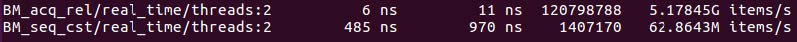
\includegraphics[width=0.9\textwidth]{content/1/chapter5/images/14.jpg}\\
Figure 5.14 – Performance of acquire-release vs. sequential consistency memory order
\end{center}

There is a lot more to the C++ memory model than just the atomic operations and the memory order. For example, when we studied false sharing earlier, we have assumed that it is safe to access adjacent elements of an array from multiple threads concurrently. It makes sense: these are different variables. And yet, it was not guaranteed by the language or even by the additional restrictions adopted by the compiler. On most hardware platforms, accessing adjacent elements of an array of integers is indeed thread-safe. But it is definitely not the case for data types of smaller size, for example, an array of bool. Many processors write a single byte using a masked integer write: they load the entire 4-byte word containing this byte, change the byte to the new value, and write the word back. Obviously, if two processors do this at the same time for two bytes that share the same 4-byte word, the second write will overwrite the first one. The C++11 memory model requires that writing into any distinct variables, such as array elements, is thread-safe if no two threads access the same variable. Prior to C++11, it was easy to write a program that would demonstrate that writing into two adjacent bool or char variables from two threads is not thread-safe. The only reason we don't have this demonstration in this book is that the compilers available today don't fall back to this aspect of C++03 behavior even if you specify the standard level as C++03 (this is not guaranteed, and a compiler could use masked writes to write single bytes in C++03 mode, but most compilers use the same instructions as in C++11 mode).

The last example of the importance of the C++ memory model also contains a valuable observation: the language and the compiler are not all that defined the memory model. The hardware has a memory model, the OS and the runtime environment have their memory models, and each component of the hardware/software system the program runs on has a memory model. The overall memory model, the total set of guarantees and restrictions available to the program, is a superposition of all of these memory models. Sometimes you can take advantage of that, for example, when writing processor-specific code. However, any portable C++ code can rely only on the memory model of the language itself, and, more often than not, other underlying memory models are a complication.

Two kinds of problems arise because of the differences in the memory model of the language and that of the hardware. First of all, there may be bugs in your program that cannot be detected on particular hardware. Consider the acquire-release protocol we used for our producer-consumer program. If we made a mistake and used the release memory order on the producer side but relaxed memory order (no barrier at all) on the consumer side, we would expect the program to produce incorrect results intermittently. However, if you run this program on an x86 CPU, it would appear to be correct. This is because the memory model of the x86 architecture is such that every store is accompanied by a release barrier, and every load has an implicit acquire barrier. Our program still has a bug, and it would trip us up if we ported it to, say, an ARM-based processor (like the one in an iPad). But the only way to find this bug on x86 hardware is with the help of a tool like the Thread Sanitizer (TSAN) available in GCC and Clang.

The second problem is the flip-side of the first one: reducing the restrictions on the memory order does not always result in better performance. As you can expect from what you have just learned, going from release to relaxed memory order on write operations does not yield any benefit on an x86 processor because the overall memory model still guarantees the release order (in theory, the compiler might do more optimizations with the relaxed memory order than with the release one, however, most compilers do not optimize the code across atomic operations at all).

The memory model provides both the scientific foundation and the common language for discussing how programs interact with the memory system. The memory barriers are the actual tools the programmer utilizes, in code, to control the memory model features. Often, these barriers are invoked implicitly by using locks, but they are always there. The optimal use of memory barriers can make a large difference in the efficiency of certain high-performance concurrent programs.














